% the following line is added to eliminate warnings about fonts on Mac
\PassOptionsToPackage{quiet}{fontspec} 

% use ctexarticle and include own package hw-cn.sty
\documentclass[]{ctexart}
\usepackage{hw-cn}

\usepackage{inputenc}
\usepackage{amsfonts,amsmath,amscd,amssymb,amsthm}
\usepackage{latexsym,bm}
\usepackage{cite}
\usepackage{mathtools,mathdots,graphicx,array}
\usepackage{fancyhdr}
\usepackage{lastpage}
\usepackage{color}
\usepackage{enumitem}
\usepackage{xcolor,tcolorbox,tikz,tkz-tab,mdframed,tikz-cd}
\usepackage{framed}
\usepackage{verbatim}
\usepackage{extarrows}
\usepackage{fontspec}
\usepackage{subfigure}
\usepackage{float} % use H command to fix position of figures
\usepackage{graphicx}
\usepackage{listings}
\usepackage{hyperref}
\usepackage{makecell}
\usepackage{diagbox}
\usepackage{bbding}


\newcommand\course{智能感知认知实践}
\newcommand\taskinfo{任务}
\newcommand\name{孙一林}
\newcommand\stuID{520030910361}

\pagestyle{fancyplain}
\headheight 25pt
\lhead{\name \\ \stuID}
\chead{\textbf{\Large 声音事件检测\taskinfo}}
\rhead{\course \\ \today}

\begin{document}

\section{提交文件简要说明}
本次实验使用超算hpc进行,代码改动集中在\texttt{model.py},并未对原有其他代码框架进行大幅更改。数据预处理根据\texttt{data}目录下的\texttt{prepare\_data.sh}文件进行,
提取的数据保存在该目录下,并未从\texttt{stu168}拷贝原始数据集(可以软链接,但并不需要)。按照原有代码框架脚本,实验结果默认保存在\texttt{experiments/Crnn}目录下,
超算运行日志保存在\texttt{slurm\_logs}文件夹下。
\section{任务理解}

\subsection{代码逻辑和声音事件检测流程理解}
整个声音事件检测流程上首先需要使用\texttt{prepare\_data.sh}脚本进行数据预处理,
将原始数据集提取并得到\texttt{feature.csv}和\texttt{label.csv}文件,这些文件即本次训练声音事件的特征和标注。
同时,还会生成元数据\texttt{class\_label\_indices.txt},以便后续训练使用。

训练时先读取config文件和log文件,之后通过元数据\texttt{class\_label\_indices.txt}
读取\texttt{dataframe},并得到dataloader,需要先实现好Crnn模块作为我们实验的模型,
之后适配优化器,得到lr\_scheduler,并进行训练。

需要注意的是,本次训练支持早停,即每个epoch都会进行validate,并计算val\_loss,
如果当前的val\_loss小于best\_loss,进行一次记录,当记录的次数达到config的阈值之后,
便认为模型的训练已经接近于收敛,这时候可以早停,得到效果不错的模型。

\subsection{弱监督情况下进行时间轴预测的难点}
对于分类任务而言,数据通常都需要带有一定的标注,不过在声音事件检测这个特定的任务场景下,大多数情况下,
我们能接触到的数据集都是不带标注或是标注不精确的,这类数据通常被称为弱标注数据。
典型的弱标注数据仅仅提供声音事件的分类,并不提供事件在时间轴上的信息,包括但不限于开始、结束时间。
由于仅提供了弱标注数据,这种监督学习可以被称为弱监督,弱监督下的声音事件检测的任务就是检测出各种事件的类别和事件的发生位置。
弱监督下的声音事件检测任务可以理解为多实例学习任务,通过将含有少量标注的大段数据看作一个大包,只知道这个包中含有某类事件,但不知道这类事件在数据包中的具体位置。

弱监督下进行时间轴预测的难点正是来源于事件在时间轴上的不精确标注。不同类型的声音事件有差异很大的声学特征,
有些声音很短,比如枪声;有些声音很长,比如说话声;还有些声音很短但是会在短时间内多次重复,比如狗吠声等等。
在弱监督的情况下,很难有一个比较好的方式去严格定义这些事件的时间边界,从而带来事件在时间轴上的混叠。
此外,生活中同一时刻通常会发生多个声音事件,即同一时刻的数据有可能是多个音元叠加的结果,在弱监督的情况下,检测的难度也会大大增加。
考虑到在声音事件检测的实际应用场景下,需要检测的声音万网距离声音收集装置很远,导致麦克风接收到的目标事件的声压级低于环境中发生的其他声音的声压级,增加了检测的难度。
由于声音相关数据集本身存在数据量少,标注困难,耗时大等特性,目前音频数据集无标注或者弱标注的数据多,强标注的数据很少,
所以目前研究弱监督下的时间轴预测仍有着比较重要的价值。

\subsection{Baseline设计的原理}
本次实验所使用的基线模型是Crnn神经网络,即所谓的卷积递归神经网络,是一种将卷积神经网络和递归神经网络结合,共同训练并推断的网络,
他可以用于在一定程度上实现对不定长的文本序列进行识别,不需要分割单个文字,而是将文本识别转化为时序依赖的序列学习问题,或者说基于图像的序列识别,并采用端到端的方式进行训练。
当然,即便对于输入图像而言,每个字符的精确位置信息不再需要了,但实际上一些对原始图像的前期裁剪工作还是必要的。

对于一个Crnn输入而言,先通过卷积神经网络对输入图像提取特征,得到特征图;
之后通过递归神经网络,比如双向LSTM,对特征序列进行预测,对序列中的每个特征向量进行学习,可以依据上下文信息做出逐帧的决策并输出预测标签分布;
最后还可以通过所谓的转录层,计算CTC损失,把从循环层获取的一系列标签分布转换成最终的标签序列。
Crnn神经网络思想的独特性在于他把卷积神经网络对图像特征提取的能力与LSTM做序列化输入识别的能力进行结合。
它既提取了图像特征,又通过序列识别避免了传统算法中难度极高的单字符切分与单字符识别,同时序列化识别也嵌入时序依赖。

\subsection{Crnn模型实现}
如下图左侧\ref{crnn1}是一个常见的crnn网络架构和输入在其中传递的流程示意。
在具体实现上,参照slides给出的模型结构\ref{crnn2},即实现了feature维度逐渐递增的五个卷积层,
并为每个卷积层适配相应的batchnorm层,辅以relu激活函数。在通过激活函数之后,还需要进行最大池化。
一共有五个最大池化层,前两个池化层窗口尺寸为$2*2$;
而最后三个池化层的窗口尺寸改为$1*2$,也就是说,图片的高度减半了五次,而宽度则只减半了三次。
使用$1*2$的池化窗口的目的是尽量保留宽度方向的信息。
在得到卷积网络部份的feature之后,将feature通过双向LSTM网络得到隐层状态,
通过sigmoid激活函数输出以得到\texttt{detection}结果。
\begin{figure}[ht]
    \centering
    \subfigure[Crnn模型流水线示意图]{
    \label{crnn1}
    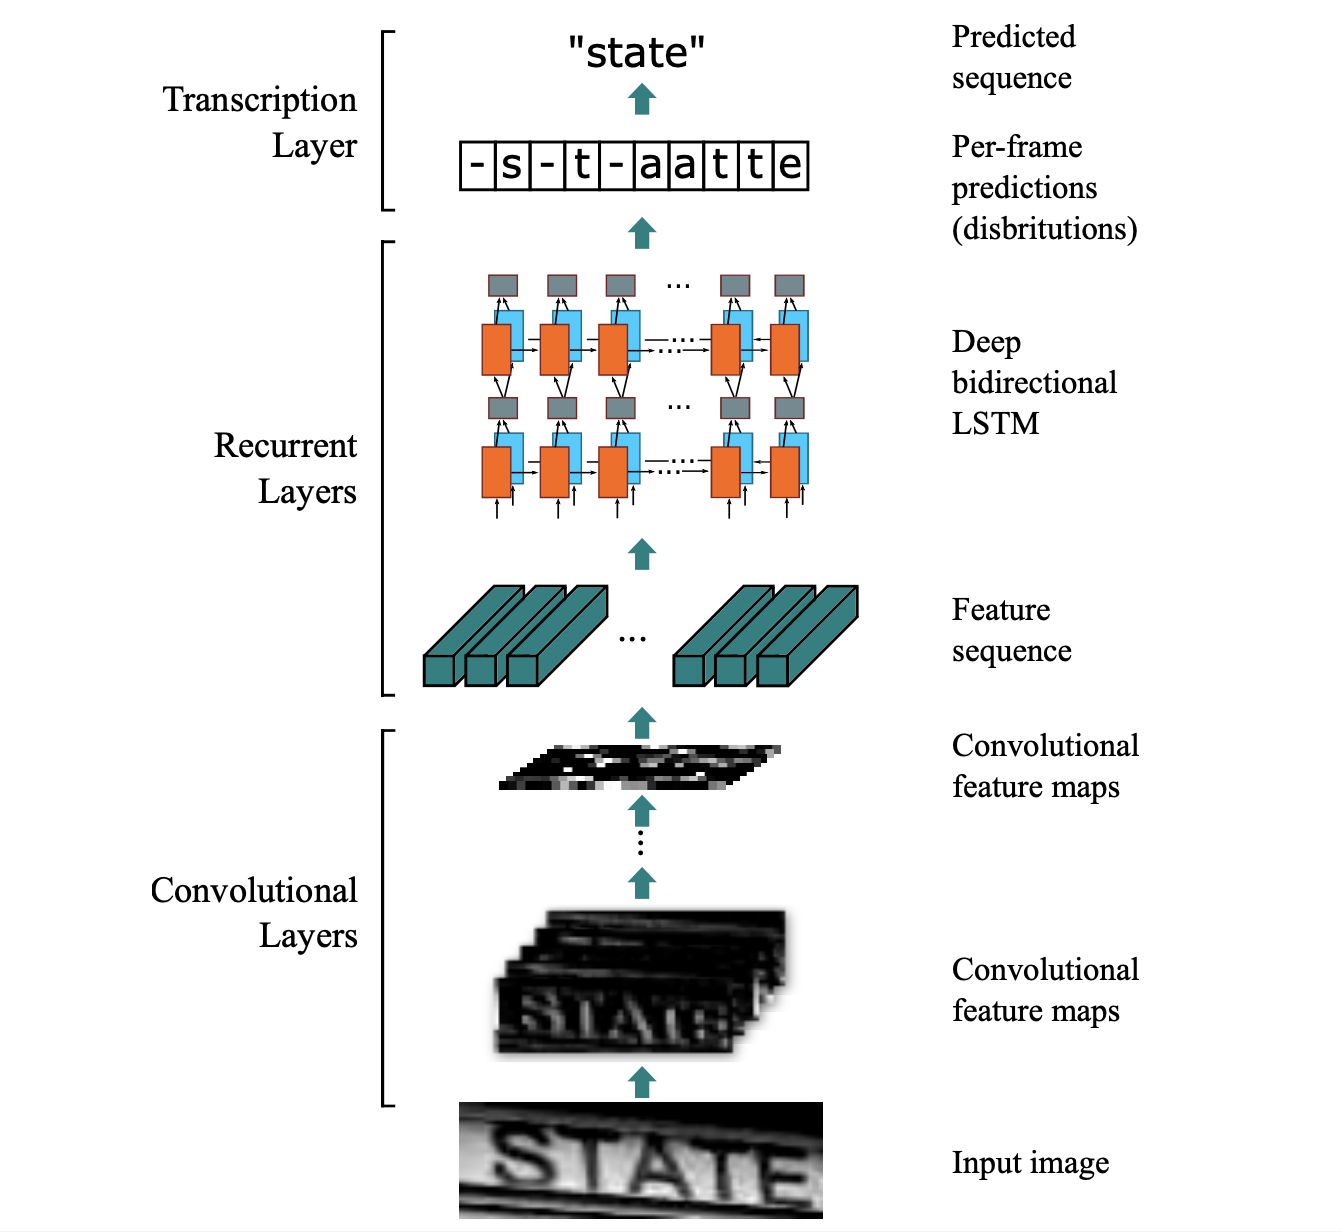
\includegraphics[width=0.5\textwidth]{asset/crnn.png}}
    \subfigure[按照slide结构的Crnn模型实现]{
    \label{crnn2}
    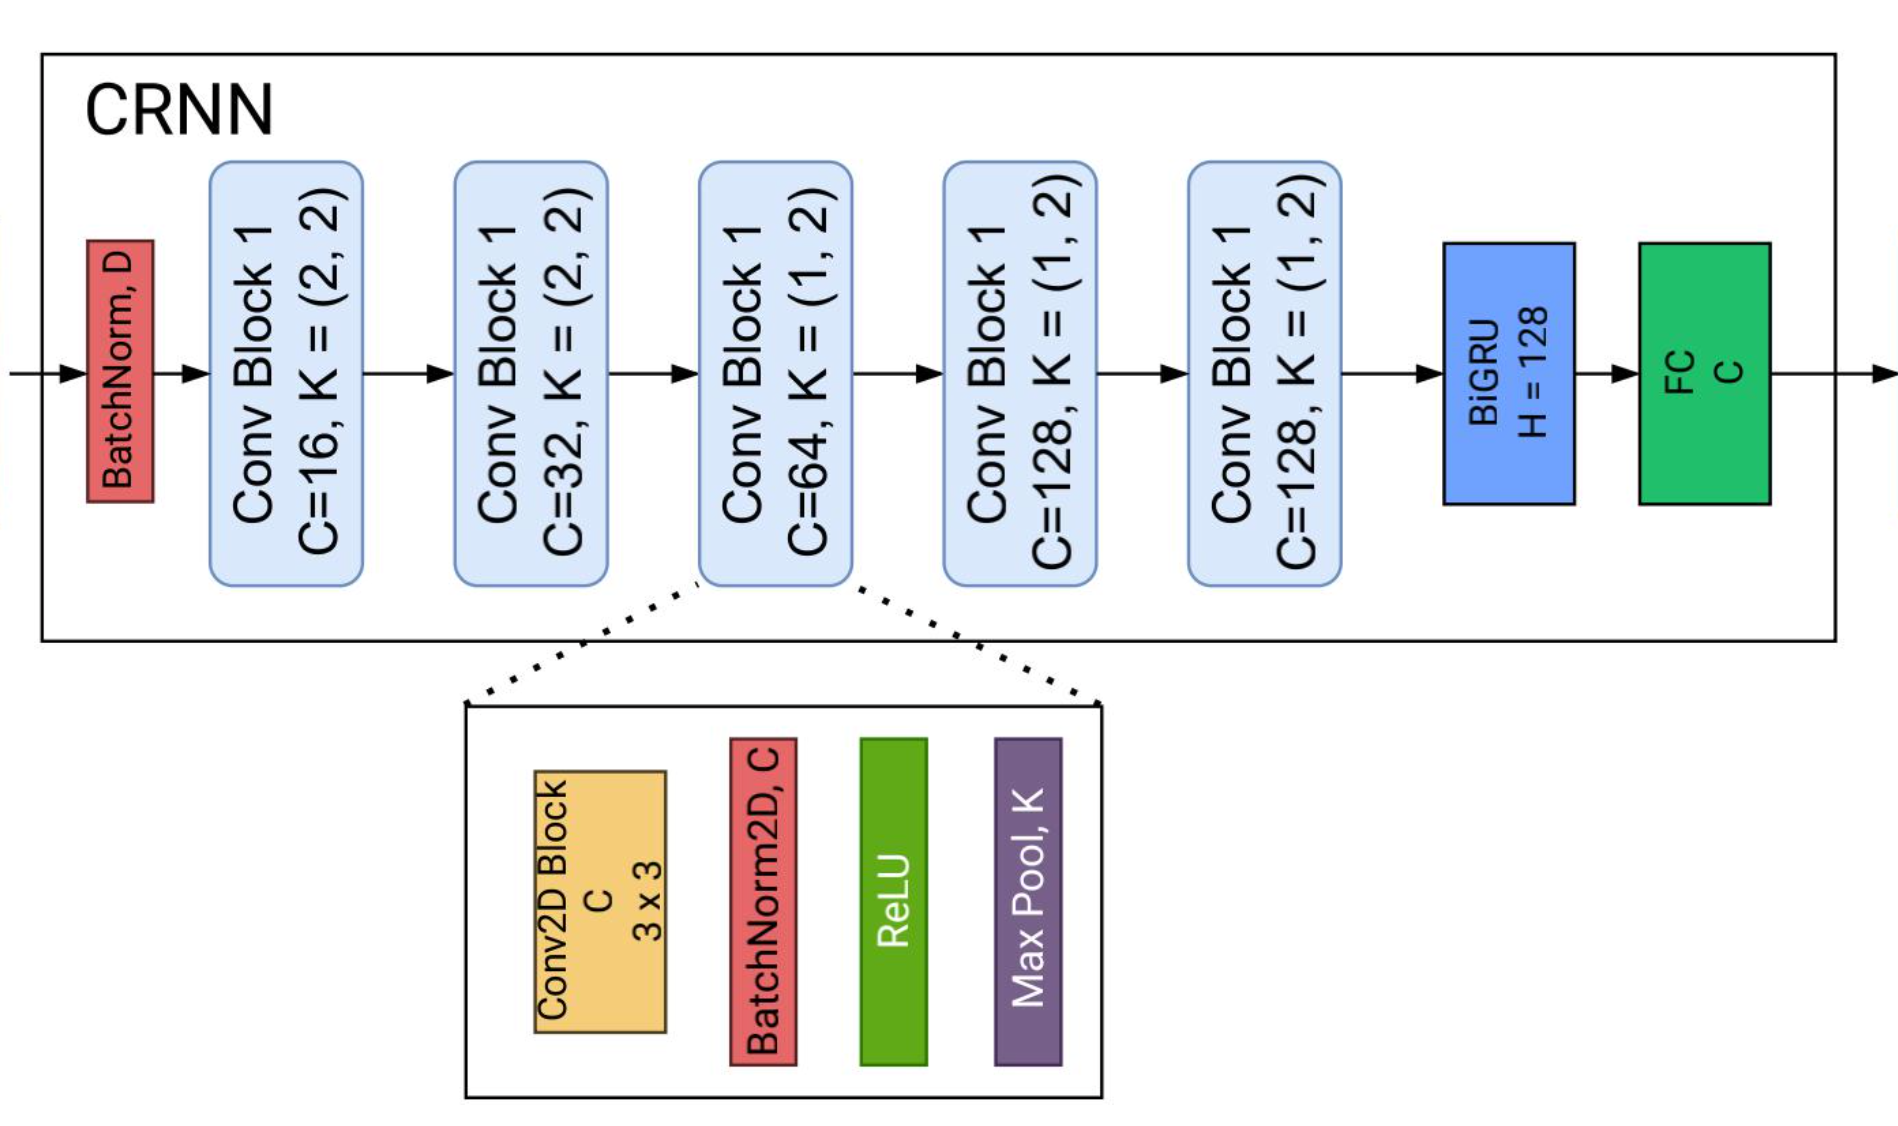
\includegraphics[width=0.45\textwidth]{asset/crnn_slide.png}}
    \caption{Crnn结构相关图片}
    \label{crnn}
\end{figure}

\newpage
\section{模型调优和实验}

\subsection{数据预处理}
将脚本cp到个人hpc目录后运行\texttt{data}文件夹下的\texttt{prepare\_data.sh}脚本,将根据\texttt{stu168}用户下的原始数据提取用于本次训练的后续相关数据。
需要使用单线程数据处理脚本,并对librosa版本降级,从而成功提取数据。
\subsection{实验结果和分析}
\texttt{baseline.yaml}中未提供大量的参数供调整,本任务的重点在于Crnn的模型搭建和结构调整,故本部分重点在于总结不同Crnn结构下的实验结果,
并展示模型结构改进对评测指标的影响。本次任务最终提交的\texttt{model.py}即保留了最优情况下的模型参数配置,其脚本则为\texttt{run.sh}及相关的配置文件。

本次实验最开始我的直观想法是直接将Crnn所需要的神经网络模块,包括但不限于fully connect, convolution, lstm, batchnorm等融合在一起,
不对参数进行细致的配置,直接使用relu, sigmoid等激活函数,在成功搭建后的初步实验结如下:
\begin{table}[ht]
    \centering
    \begin{tabular}{|l|cll|}
    \hline
    Metrics        & \multicolumn{1}{c|}{f\_measure} & \multicolumn{1}{l|}{precision}  & recall     \\ \hline
    event\_based   & \multicolumn{1}{c|}{0.00743036} & \multicolumn{1}{l|}{0.00666628} & 0.00990206 \\ \hline
    segment\_based & \multicolumn{1}{c|}{0.196863}   & \multicolumn{1}{l|}{0.310598}   & 0.161337   \\ \hline
    tagging\_based & \multicolumn{1}{c|}{0.449451}   & \multicolumn{1}{l|}{0.568862}   & 0.387041   \\ \hline
    mAP            & \multicolumn{3}{c|}{0.5058306091886279}                                        \\ \hline
    \end{tabular}
    \caption{简单Crnn结构:双层卷积}
    \label{exp1}
\end{table}

初步实验成功之后,进行模型结构调整,增加卷积层和BatchNorm层的个数,使用两种不同的池化方式,结果如下:
\begin{table}[ht]
    \centering
    \begin{tabular}{|l|cll|}
    \hline
    Metrics        & \multicolumn{1}{c|}{f\_measure} & \multicolumn{1}{l|}{precision}  & recall     \\ \hline
    event\_based   & \multicolumn{1}{c|}{0.00831543} & \multicolumn{1}{l|}{0.0116714}  & 0.00656456 \\ \hline
    segment\_based & \multicolumn{1}{c|}{0.226929}   & \multicolumn{1}{l|}{0.42916}    & 0.156146   \\ \hline
    tagging\_based & \multicolumn{1}{c|}{0.553278}   & \multicolumn{1}{l|}{0.630679}   & 0.511583   \\ \hline
    mAP            & \multicolumn{3}{c|}{mAP: 0.5788640257440317}                                        \\ \hline
    \end{tabular}
    \caption{改进Crnn结构:三层卷积、batchnorm、两种pooling}
    \label{exp2}
\end{table}

\newpage
按照slides给出模型结构进行最终改进(此即提交文件中的模型结构),结果如下:
\begin{table}[ht]
    \centering
    \begin{tabular}{|l|cll|}
    \hline
    Metrics        & \multicolumn{1}{c|}{f\_measure} & \multicolumn{1}{l|}{precision}  & recall     \\ \hline
    event\_based   & \multicolumn{1}{c|}{0.0108622}  & \multicolumn{1}{l|}{0.0139943}  & 0.00960896 \\ \hline
    segment\_based & \multicolumn{1}{c|}{0.231898}   & \multicolumn{1}{l|}{0.418706}   & 0.163764   \\ \hline
    tagging\_based & \multicolumn{1}{c|}{0.582452}   & \multicolumn{1}{l|}{0.628041}   & 0.565621   \\ \hline
    mAP            & \multicolumn{3}{c|}{mAP: 0.6098265732798768}                                        \\ \hline
    \end{tabular}
    \caption{最终Crnn结构:模型结构保留在model.py中}
    \label{exp3}
\end{table}

模型结构确定,继续进行参数调整,包括但不限于各个卷积层的in\_channels, out\_channels, LSTM网络的隐层维度、层数(即提交文件中的默认参数),
主要是增大卷积层channel的个数和LSTM网络隐层向量的维度,结果如下:
\begin{table}[ht]
    \centering
    \begin{tabular}{|l|cll|}
    \hline
    Metrics        & \multicolumn{1}{c|}{f\_measure} & \multicolumn{1}{l|}{precision}  & recall     \\ \hline
    event\_based   & \multicolumn{1}{c|}{0.00938473} & \multicolumn{1}{l|}{0.0115726}  & 0.00811011 \\ \hline
    segment\_based & \multicolumn{1}{c|}{0.240401}   & \multicolumn{1}{l|}{0.423576}   & 0.172586   \\ \hline
    tagging\_based & \multicolumn{1}{c|}{0.633284}   & \multicolumn{1}{l|}{0.637923}   & 0.634307   \\ \hline
    mAP            & \multicolumn{3}{c|}{mAP: 0.6330678570776226}                                        \\ \hline
    \end{tabular}
    \caption{最终Crnn参数:模型参数是model.py中的默认参数}
    \label{exp4}
\end{table}

可以看到,对于声音事件检测而言,卷积层部分的模型结构和参数确实
能够对后续的实验结果产生比较重要的影响,这再一次说明卷积神经网络的结构和范式
也能对声音事件检测有着启发意义。
\end{document}